\documentclass[letter,11pt]{article}
\usepackage[pdftex]{graphicx}
\usepackage{float}
\usepackage{amsmath}
\begin{document}
	\begin{center}
		\Large\textbf{CSCI 567-Machine Learning Assignment-4}
	\end{center}
	
	\section{Neural Network}
	\begin{equation}
	\mathcal{L}(x,\hat{x}) = \frac{1}{2}((x_1 - \hat{x}_1)^2 + (x_2 - \hat{x}_2)^2) + (x_3 - \hat{x}_3)^2)
	\end{equation}
	\begin{equation}
	\mathcal{L}(y,\hat{y}) = \frac{1}{2}((y_1 - \hat{y}_1)^2 + (y_2 - \hat{y}_2)^2)
	\end{equation}
	
	$$ \frac{\partial \mathcal{L}(y,\hat{y})}{\partial v_{jk}} =   \frac{\partial \mathcal{L}(y,\hat{y})}{\partial y}   \frac{\partial y}{\partial v_{jk}} = (-y + \hat{y})z $$
	$$  \frac{\partial \mathcal{L}(y,\hat{y})}{\partial y} = \frac{1}{2} (-2y + 2\hat{y}) = -y + \hat{y}$$
	$$ \frac{\partial y}{\partial v_{jk}} = \frac{\partial}{\partial v_{jk}} \sum_{k} v_{jk}z_k$$
	\begin{equation}
	\frac{\partial \mathcal{L}(y,\hat{y})}{\partial v_{jk}} =(-y_j + \hat{y}_j)z_k
	\end{equation}
	
	$$\frac{\partial \mathcal{L}(y,\hat{y})}{\partial w_{ki}} =  \frac{\partial \mathcal{L}(y,\hat{y})}{\partial y} \frac{\partial y}{\partial z} \frac{\partial z}{\partial P_1} \frac{\partial P_1}{\partial w_{ki}}$$ 
	$$  \frac{\partial \mathcal{L}(y,\hat{y})}{\partial y} = \frac{1}{2} (-2y + 2\hat{y}) = -y + \hat{y}$$
	$$  \frac{\partial z}{\partial P_1} = z(1-z)$$
	$$ \frac{\partial y}{\partial z} = v $$
	$$ \frac{\partial P_1}{\partial w_{ki}} = \tilde{x}$$
    \begin{equation}
	\frac{\partial \mathcal{L}(y,\hat{y})}{\partial w_{ki}} = (-y + \hat{y})vz(1-z)\tilde{x}
	\end{equation}
	$$\frac{\partial \mathcal{L}(x,\hat{x})}{\partial w_{ki}} =  \frac{\partial \mathcal{L}(x,\hat{x})}{\partial \hat{x}} \frac{\partial \hat{x}}{\partial w_{ki}}$$ 		
    $$  \frac{\partial \mathcal{L}(x,\hat{x})}{\partial \hat{x}} = \frac{\partial}{\partial w_{ki}} w^Tz = z + \frac{\partial z}{\partial w} = z + z(1-z) \tilde{x} $$
    $$ \frac{\partial z}{\partial w} = \frac{\partial z}{\partial P_1} \frac{\partial P_1}{\partial w} = z(1-z)\tilde{x}$$
    \begin{equation}
    \frac{\partial \mathcal{L}(x,\hat{x})}{\partial w_{ki}} = (-x + \hat{x})(z+z(1-z)\tilde{x})
    \end{equation}
        
        Backpropagation update for $v_{jk}$ (where $\eta_1$ is the step length in steepest descent):
        
        $$ v_{jk}^{t+1} = v_{jk}^{t} -\eta_1(-y+\hat{y})z $$
        Backpropagation update for $w_{ki}$:
        
        $$  w_{ki}^{t+1} = w_{ki}^{t} -\eta_2  ((-y + \hat{y})vz(1-z)\tilde{x}) -\eta_3 ((-x + \hat{x})(z+z(1-z)\tilde{x}))$$
        
	\section{Mixture Model and EM Algorithm}
	
	\subsection{Log-Likelihood}
	$X_i$ values are unknown for the last $n-r$ variables. Let's call them $U_i$ for now. For rest $X_i = y_i$.
	$$ log P(x,\lambda) = \sum_{i = 1}^{r}(log \lambda - \lambda X_i) + \sum_{i = r+1}^{n} (log \lambda - \lambda U_i) = \sum_{i = 1}^{n} log \lambda - \lambda(\sum_{i =1}^{r} y_i + \sum_{i = r+1}^{n} U_i)$$
	\subsection{E-Step}
	
	We will use the expectation for the last $n-r$ variable. Exponential distribution has a memoryless property. We know that each $U$ exponential random value did not happen until $c_i$. Than their expectation is:
	$$ E(U_i) = c_i + \frac{1}{\lambda} $$
	
	\subsection{M-Step}
	$$E[log P(x,\lambda)] = E[\sum_{i = 1}^{n} log \lambda - \lambda(\sum_{i =1}^{r} y_i + \sum_{i = r+1}^{n} U_i)]$$
	$$ = n \log \lambda -\lambda \sum_{i = 1}^{r} y_i - (n-r)\lambda (c_i + \frac{1}{\lambda} )= n \log \lambda -\lambda \sum_{i = 1}^{r} y_i - n\lambda c_i - n +r \lambda c_i + r$$
	
	$$\frac{\partial E[log P(x,\lambda)]}{\partial \lambda} = \frac{n}{\lambda} - \sum_{i=1}^{r} y_i - nc_i + rc_i = 0$$
	\begin{equation}
	\lambda = \frac{n}{\sum_{i = 1}^{r} y_i + (n-r)c_i}
	\end{equation}
		\section{K-Means}
		
	 \section{Programming Questions}
	 \subsection{K-Means}
	 	\begin{figure}[H]%                 use [hb] only if necceccary!
	 	\centering
	 	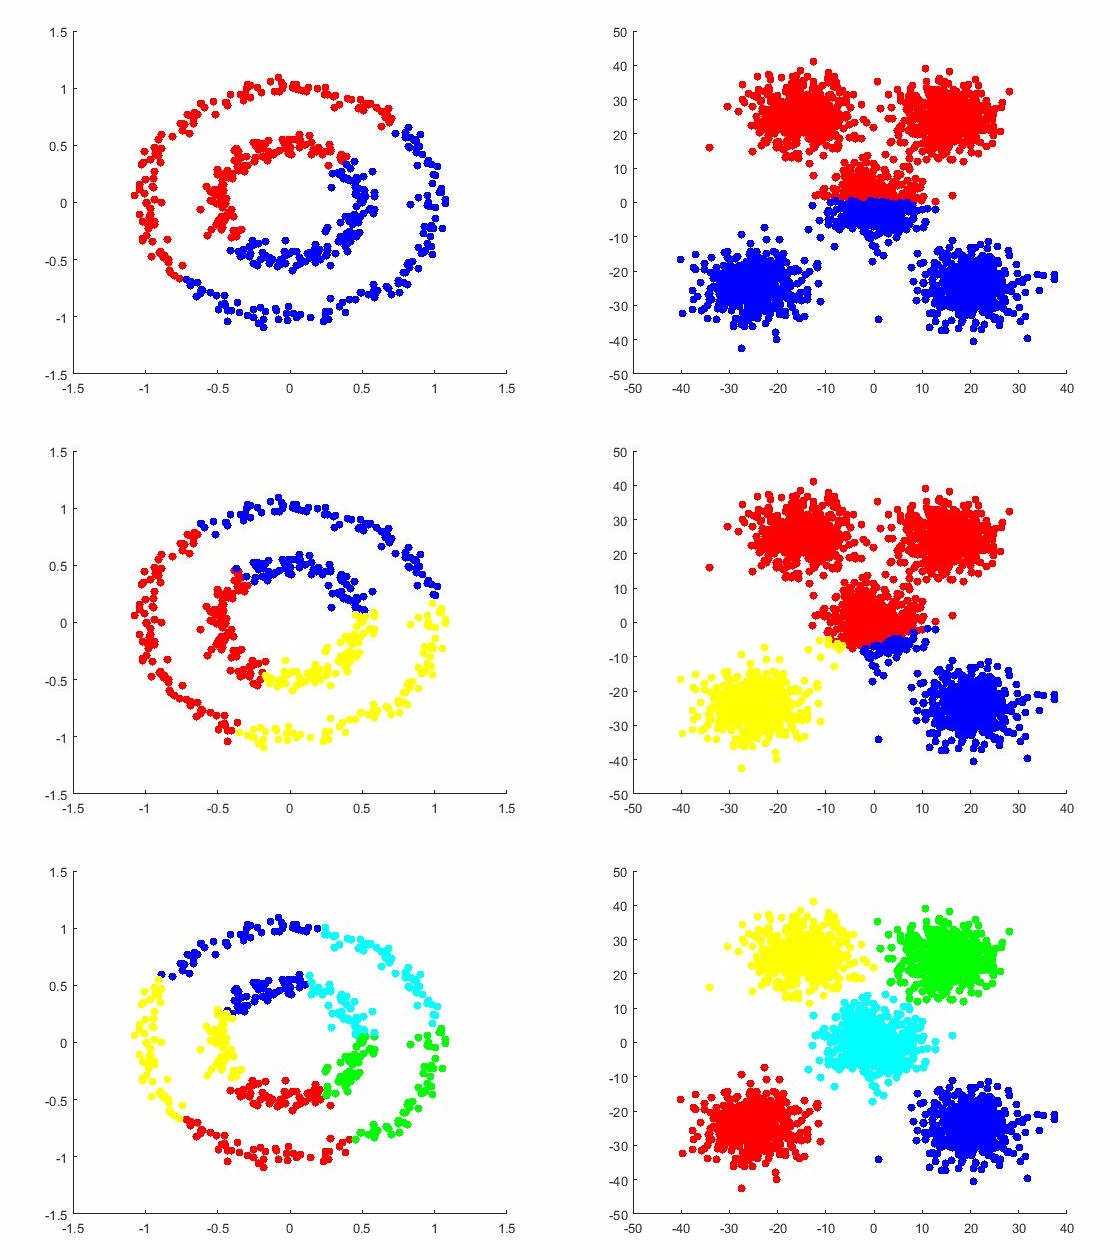
\includegraphics[width=9cm]{C:/Users/okazk_000/Desktop/Spring 2016/CSCI 567/HW4/Kmeans.jpg}
	 	\caption{K-Means algorithm over 2 different dataset}
	 	\label{fig:test}
	 	\end{figure}
	 	
	 	It can't separate two circles no matter K is 2,3, or 5. This is because K-Means uses distance metric and it can't figure out the shapes. It just classifies the data points that are close o each other.
	 
	 \subsection{Mixture of Gaussian Distributions with Unknown Component Numbers} 
	
			\begin{center}
			\begin{tabular}{|c| c |c |c|} 
				\hline
				Number of Components & Best Heldout & Training Log Likelihood & Number Until Convergence \\ [0.5ex] 
				\hline
				3 & -4879.4 & -1786.4 & 85 \\ 
				\hline
				5 & -4784.8 & -1770.3 & 190 \\
				\hline
				7 & -5224.4 & -1896 & 150 \\
				\hline
				9 & -5397.6 & -1932.9 & 151 \\
				\hline
				11 & -5474.4 & -1941.2 & 310 \\
				\hline
			\end{tabular} \\

		\end{center}
			
				Table 1: Best Heldout and Training log Likelihood Values\\
		
				Since it has the maximum log-likelihood value for both Heldout and Training data, I would choose 5 Components .
			 \subsection{Vector Quantization Using k-means} 
			 \noindent
			 \parbox{2cm}{}%
			 \hfill
			 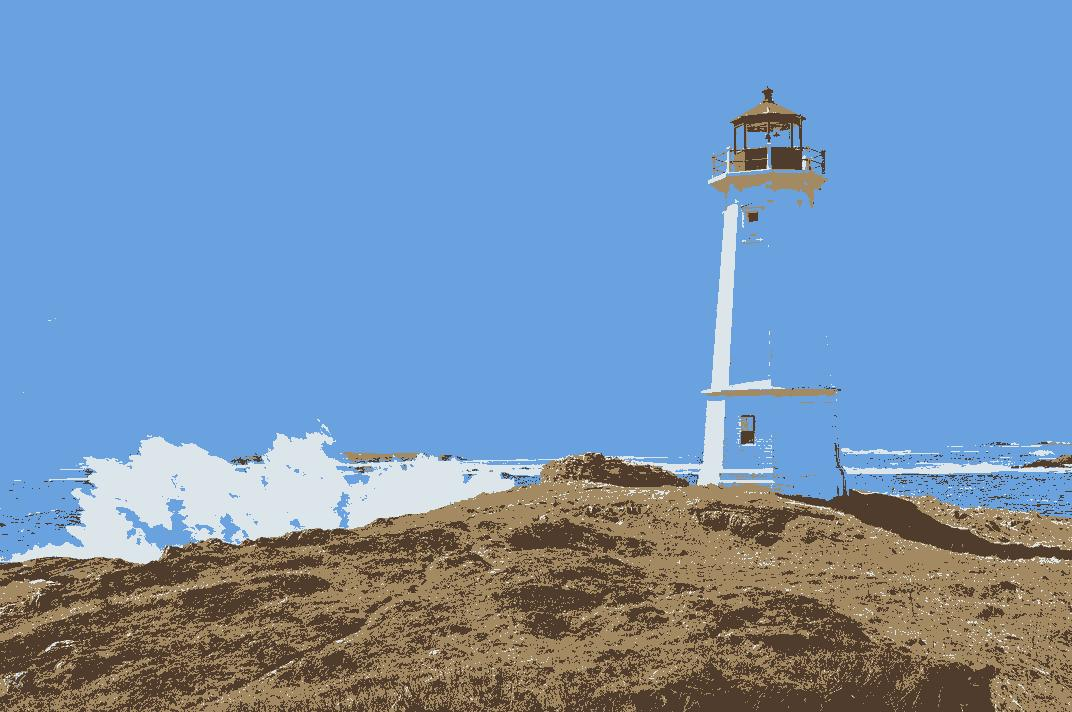
\includegraphics[width=13.5cm]{C:/image4cluster.jpg}
			 \centering
			 Figure-1: K = 4
			 \noindent
			 \parbox{0.5cm}{}%
			 \hfill
			 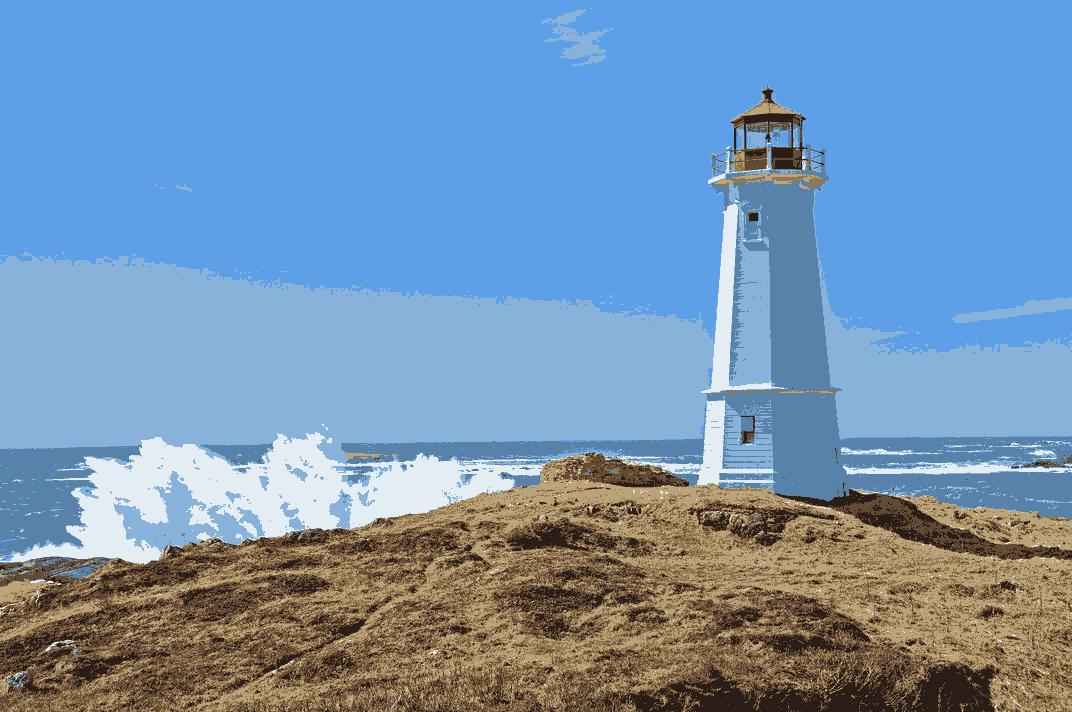
\includegraphics[width=13.5cm]{C:/image8cluster.jpg}
			 \centering
			 Figure-2: K = 8	
			 \noindent
			 \parbox{0.5cm}{}%
			 \hfill
			 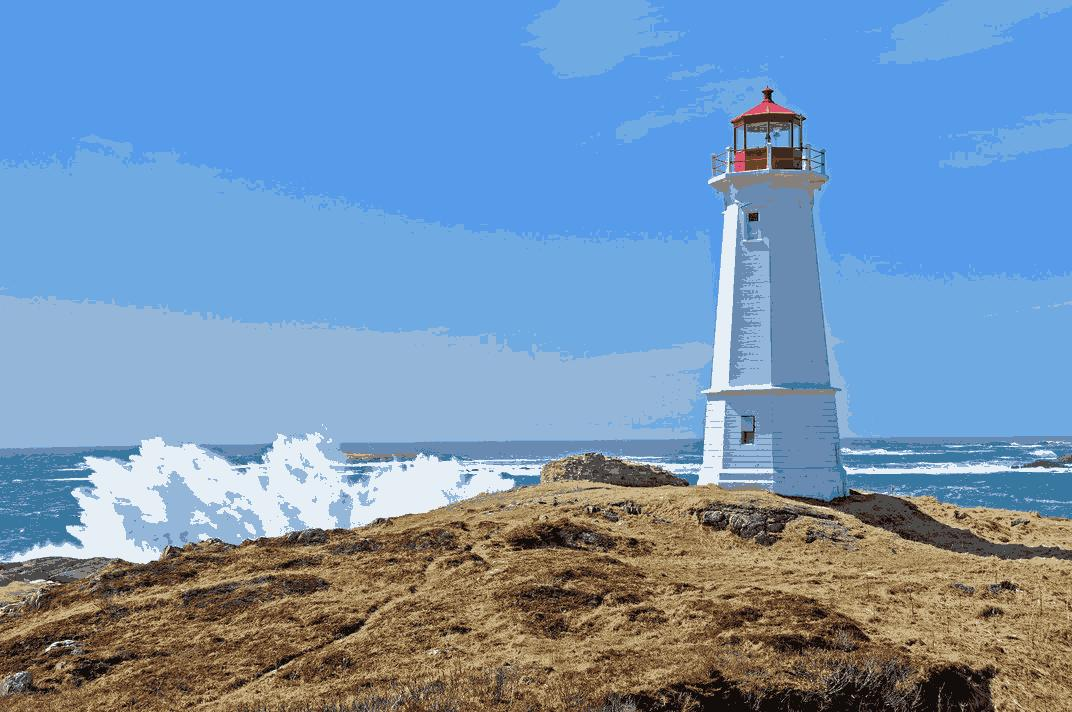
\includegraphics[width=13.5cm]{C:/image24cluster.jpg}
			 \centering
			 Figure-3: K = 24			 


								
\end{document}